\documentclass{book}
\usepackage{graphicx}
\usepackage{color}
\usepackage{url}
\usepackage{amssymb}
\usepackage{appendix}
\usepackage[hidelinks]{hyperref}
\usepackage{fontspec}	% To change default font
%\usepackage{fancyhdr}	%to include customized footer and header
%\pagestyle{fancy}
%\lhead{}
%\chead{\leftmark}
\graphicspath{{./Figures/}}
\setmainfont{URW Palladio L} % Use if font is to be set

\begin{document}
%-----------------------------------
% For customised Title Page
\thispagestyle{empty}
%\input{./title.tex} %Cover page
\thispagestyle{empty}
%\input{./inner.tex}	%Inner title page
%--------------------------------------------------------------------

%Default Title page 
\title{Analog Communication
Laboratory Manual}
\date{December 2013}
\author {Authors: Contributor-1, Contributor-2...}
\maketitle
%----------------------------------------------------------
%\thispagestyle{empty}
  
\textcopyright{}2013
\\[5cm]
    This work is licensed under a Creative Commons Attribution-Share Alike 4.0 India License. See \url{http://creativecommons.org/licenses/by-sa/4.0/} for more details.
%------------------------------------------------------------






\thispagestyle{empty}
\tableofcontents
\thispagestyle{empty}
\thispagestyle{empty}

\listoffigures
\thispagestyle{empty}
\chapter [Introduction to Analog Communication]{Introduction to Analog Communication}


\cite{ACmanual}Communication is the transfer of information from one place to another. A bidirectional communication system operates in opposite directions. The receiver can respond
to the sender. Radio communication uses electrical energy to transmit information. Because electrical energy travels almost as fast as light, radio communication is essentially instantaneous.
A radio transmitter converts audio (sound) signals to electrical signals that are sent over wires or through space. A radio receiver converts the electromagnetic waves back to sound waves so that the
information can be understood. 

The transmitted information is the \textbf {intelligence signal} or \textbf{ message signal}.
 Message signals are in the \textbf {Audio Frequency (AF)} range of low frequencies from about 20 Hz to 20 kHz.
 
 
The \textbf{Radio Frequency (RF)}  is the carrier signal. Carrier signals have high frequencies that range from 10 kHz up to about 1000 GHz.
A radio transmitter sends the low frequency message signal at the higher carrier signal frequency by combining the message signal with the carrier signal.

\textbf{Modulation} is the process of changing a characteristic of the carrier signal with the message
signal. In the transmitter, the message signal modulates the carrier signal.
The modulated carrier signal is sent to the receiver where \textbf{demodulation} of the carrier occurs to
recover the message signal.\\[10pt]
\textsc{\textbf {IMPORTANT TERMS}}
\begin{itemize}
\item \textbf{Audio} - signals that a person can hear.

\item \textbf{Electromagnetic waves} - the radiant energy produced by oscillation of an electric
charge.

\item \textbf{Intelligence signal} - any signal that contains information; it is also called the
message signal.
\item \textbf{Message signal} - any signal that contains information; it is also called
the intelligence signal. 
\item \textbf{Audio Frequency (AF)} - frequencies that a person can hear.
AF signals range from about 20 Hz to 20 kHz.
\item \textbf{Radio Frequency (RF)} - the transmission frequency of electromagnetic (radio) signals.
RF frequencies are from about 300 kHz to the 1,000,000 kHz range.
\item \textbf{Carrier signal} - a single, high-frequency signal that can be modulated by a message
signal and transmitted.
\item \textbf{Modulation} - the process of combining the message signal with the carrier signal that
causes the message signal to vary a characteristic of the carrier signal.
\item \textbf{Demodulation} - the process of recovering or detecting the message signal from the
modulated carrier frequency.
\item \textbf{Amplitude Modulation (AM)} - the process of combining the message signal with
the carrier signal and the two sidebands: the lower sideband and the upper
sideband.
\item \textbf{Frequency Modulation (FM)} - the process of combining the message signal with
the carrier signal that causes the message signal to vary the frequency of the
carrier signal.
\item \textbf{Phase Modulation (PM)} - the process of combining the message signal with the
carrier signal that causes the message signal to vary the phase of the carrier signal.
\item \textbf{Angle modulation} - the process of combining the message signal with the carrier signal that causes the message signal to vary the frequency and/or phase of the
carrier signal.
\item \textbf{Balanced modulator} - an amplitude modulator that can be adjusted to control the
amount of modulation.
\item \textbf{Double-Sideband (DSB)} - an amplitude modulated signal in which the carrier is
suppressed, leaving only the two sidebands: the lower sideband and the upper
sideband.
\item \textbf{Mixer}- an electronic circuit that combines two frequencies.
\item \textbf{Product detector} - a detector whose audio frequency output is equal to the product of the
Beat
Frequency Oscillator (BFO) and the RF signal inputs.
\item \textbf{Phase detector} - an electronic circuit whose output varies with the phase differential
of the two input signals.
\item \textbf{Envelopes}- the waveform of the amplitude variations of an amplitude modulated
signal. 
\item \textbf{Sidebands} - the frequency bands on each side of the carrier frequency that
are formed during modulation; the sideband frequencies contain the intelligence of
the message signal.
\item \textbf{AM} - an amplitude modulated signal that contains the carrier signal and the two
sidebands: the lower sideband and the upper sideband.
\item \textbf{Bandwidth} - the frequency range, in hertz (Hz), between the upper and lower
frequency limits. 
\item \textbf{Harmonics} - signals with frequencies that are an integral multiple of
the fundamental frequency. 
\item \textbf{Beat Frequency Oscillator (BFO)} - an oscillator whose
output frequency is approximately equal to the transmitter's carrier frequency and is
input to a product detector
\end {itemize}
%CHAPTER-----------------------------------------------------------------------
\chapter[Intermediate Frequency Amplifier]{Intermediate Frequency (Tuned) Amplifier}
%-------------------
\section*{Aim}
To design and implement a tuned  intermediate frequency amplifier using BJT and IFT.
%--------------------
\section*{Theory}


A tuned amplifier is same as a normal voltage amplifiers except that they are designed to amplify signals of a particular frequency and reject signals of all other frequencies.

A tuned load is to be inevitably used in the amplifier circuit to make the gain maximum at some particular frequency. The presence of tuned load eliminates the need for biasing BJT in the active region, because it can provide full sinusoidal swing of the output voltage even if the active element conducts only during a fraction of the sinusoidal cycle. The tuned circuit resonates at one frequency and so the unwanted frequencies are suppressed, and the wanted full signal (sine wave) is extracted by the tuned load.\footnote{\url{http://en.wikipedia.org/wiki/Electronic_amplifier\#Class_C}}

The circuit here is a single tuned Class-C amplifier. An intermediate frequency transformer(IFT) is used as tuned load. IFT is tuned to standard 455 kHz audio frequency. (See \ref{IFT})

The Class-C operation reduces power dissipation in the active device. When the input signal is at the frequency of 455 kHz, the current pulses at that frequency are fed to the tuned load which makes them oscillate at that frequency. Thus full sinusoidal voltage waveform is generated across the load resistor.

\section*{Design}
%-----------------
\textcolor{red}{Design equations need to be verified}
Let the required output be $V_{pp}$ sine wave.
Let the intermediate frequency for which the circuit is tuned is 455 kHz.
Use high frequency transistor BF195.
\begin{equation}
I_c=10 \% \ of \  I_{Cmax} =\  1mA
\end{equation}
\noindent Let $V_{CC}$ be 20\% more than the output,ie. 10V.
\begin{equation}
V_{CC}=\ 12 \ V
\end{equation}
For class C mode of operation set $V_{CE}$ = 10 V.Hence $V_{RE}=2V$. Now the BJT is biased at cut-off.
\begin{equation}
V_{RE}=I_{E}. R_E
\end{equation}
\begin{equation}
I_E \approx I_C 
 \end{equation}
\noindent Hence
 \begin{equation}
I_E = 1mA
\end{equation}
\noindent Thus
\begin{equation}
R_E=\frac{V_{RE}}{I_E}=\frac{2V}{1mA}=2k\Omega
\end{equation}
\subsubsection{Design of Resistors $R_1$ and $R_2$}

 \noindent Since the transistor is in cut-off, $V_{BE}$ = 0 V. Hence,
 \begin{equation}
V_{R2}=\ V_{BE}+V_{RE} =\ 0+2V= 2V
\end{equation}
\noindent Let $I_2 =\ 9 I_B$ and $I_1=\ 10I_B$
\begin{equation}
I_B=\frac{I_C}{h_{FE}}=\frac{1mA}{67}=\ 14.9 \mu A.
\end{equation}
\begin{equation}
V_{R2}=R_2I_2 
\end{equation}

\begin{equation}
\therefore R_2=\frac{V_{R2}}{I_2}\\ 
= \frac{2}{9X14.9\mu A} =14.9 k\Omega \approx 12 k\Omega
\end{equation}
\begin{equation}
V_{R1}= V_{CC}-V_{R2} =12V-2V=10V
\end{equation}

\begin{equation}
R_1=\frac{V_{R1}}{10I_B} =\frac{10V}{10X14.9\mu A}=67k\Omega
\end{equation}
\subsubsection{Design of capacitors}
The reactance of input coupling capacitor should be such that,
\begin{equation}
X_{C1} \leq \frac{R_{in}}{10}
\end{equation}
\begin{equation}
R_{in}= R_1 ||R_2 || h_{FE}r_e
\end{equation}
\section*{Circuit Diagram}
\section*{Procedure}
\section*{Observation}
\section*{Result}

\chapter[Amplitude Modulation- Generation]{Amplitude Modulation- Generation}

\section*{Aim}
To design and set-up  an AM generator using BJT and measure the modulation index from the observed output waveform.

\section*{Theory}
\paragraph{}
	The transistor $T_1$ is configured as a common emitter amplifier. The RF carrier wave is given at the base through a coupling capacitor $C_1$.  The message signal used for modulation is the AF signal applied between the emitter resistance and the ground. The message signal modulates the envelope of the carrier which is obtained as output from the collector through a coupling capacitor $C_3$. 
\paragraph{}
The ratio of the maximum amplitude of the modulating signal voltage to that of the carrier voltage is termed as modulation index. This is represented as $m=\frac{V_m}{V_c}$.


\section*{Design}
\textcolor{red}{Design steps need to be verified}

\paragraph{DC Biasing conditions:}
Choose BF194 which is a high frequency transistor. From its datasheet (See \ref{BF194/195}) the various parameters can be obtained as:

 
Let the supply voltage be 60\% of the maximum $V_{ce}$.  \begin{equation}
V_{cc}=\ 60\% of V_{cemax}=\ 12 V
\end{equation}

\noindent Let the collector current $I_c$ be 10\% of maximum rated value.
\begin{equation}
I_{c}=\ 3\% \ of \ I_{cmax}=\ 1 mA
\end{equation}

\noindent In-order to fix the biasing point in the middle of load line, let $V_{RC}$ be 40\% of $V_{cc}$, $V_{RE}$\ be\ 10\% \ of $V_{cc}$ and $V_{ce}$\  be\ 50\% \ of $V_{cc}$.
\begin{equation}
V_{RC}=\ 45\% \ of \ V_{cc}=\ 5.4V
\end{equation}
\begin{equation}
V_{RE}=\ 5\% \ of \ V_{cc}=\ 0.6V
\end{equation}
\begin{equation}
V_{ce}=\ 50\% \ of \ V_{cc}=\ 6V
\end{equation}
\paragraph{Design of Resistors:}
\begin{equation}
R_C=\frac{V_{RC}}{I_c}=\ \frac{5.4V}{1mA}=\ 5.4 k\Omega
\end{equation}
\begin{equation}
R_E=\frac{V_{RE}}{I_e}=\ \frac{0.6V}{1mA}=\ 600\Omega
\end{equation}
\noindent From the datasheet, hFE has a minium value of 67. 
\begin{equation}
I_b=\frac{I_c}{hFE}=\frac{1mA}{67}=\ 15 \mu A
\end{equation}
\noindent Assume the current through $R_1=\ 10 I_b$ and that through $R_2=9I_b$ 
\begin{equation}
 V_{R2}=V_{be}+V_{RE}\\ =0.7+0.6V=1.3V
\end{equation}
\noindent Then
\begin{equation}
R_2=\frac{V_{R2}}{9I_b}=\frac{1.2V}{9X15X10^{-6}}=8.8 k\Omega
\end{equation}
\noindent and 
\begin{equation}
R_1=\frac{V_{R1}}{10I_b}=\frac{10.8V}{10X15X10{^-6}}= 72k\Omega
\end{equation}

\noindent Based on these design equations use the standard resistor values of $R_1=22k\Omega,\ R_2=10k\Omega, \ R_c=10k\Omega,\ R_c=560\Omega$ and a load resistance of $R_L=1k\Omega$.
Use coupling capacitors $C_1=0.1 \mu F,\ C_2=0.001\mu F$ and emitter bye-pass capacitor $C_E=0.01\mu F$.
\subsection*{Components and Equipments Required}
Function Generators(2), CRO(2), Connection wires, Breadboard, Probes.
\\BF194 - High frequency bipolar junction transistor
\\ $22k\Omega,\  10k\Omega\ (2),\ 560\Omega,\,\ 1k\Omega $ - Resistors
\\ $ 0.1\mu F,\ 0.01\mu F, \ 0.001\mu F $ - Capacitors
\\ 
\section*{Circuit Diagram}
\begin{figure}[h]
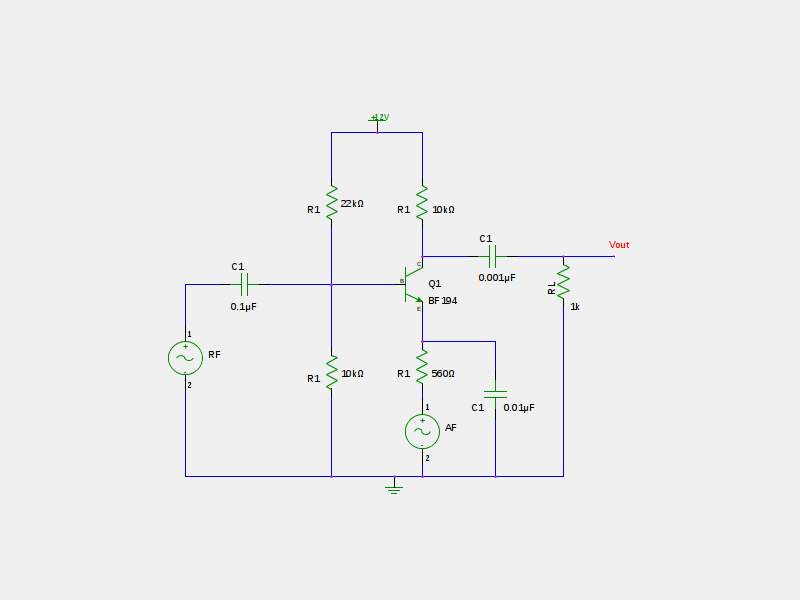
\includegraphics[width=15cm, height=10cm, trim=5cm 3.5cm 4cm 3.5cm, clip=true]{AM.png}
\caption{Circuit Diagram for Amplitude modulation using BJT}

\end{figure}

\section*{Procedure}
\begin{enumerate}
\item
Set up the circuit after verifying the condition of components.
\item
Feed AF modulating signal (say, $f_m=1kHz$ and $E_m=150mV$) and Rf carrier (say, $f_c=70kHz$ and $E_c=300mV$) using function generators.
\item
Adjust amplitude and frequencies of the AF and RF signals and observe amplitude modulated waveform on the CRO.
\item
Fix $f_m$ and $f_c$. Note down $E_{max}$ and $E_{min}$ of the AM signal and calculate modulation index according to the formula ,
\begin{equation}
m=\frac{E_{max}-E_{min}}{E_{max}+E_{min}}.
\end{equation}
Here $E_{max}$ is the maximum of the positive envelope of the carrier and $E_{min}$ is the minimum of the positivee envelope of the carrier.
\item
Repeat for different values of $E_m$ and $E_c$. Observe the AM waveforms for different values of m.
\item
Plot the waveforms on a graph sheet.
\item

Fill in the observation column
\end{enumerate}


\section*{Observation}

\begin{figure}[h]

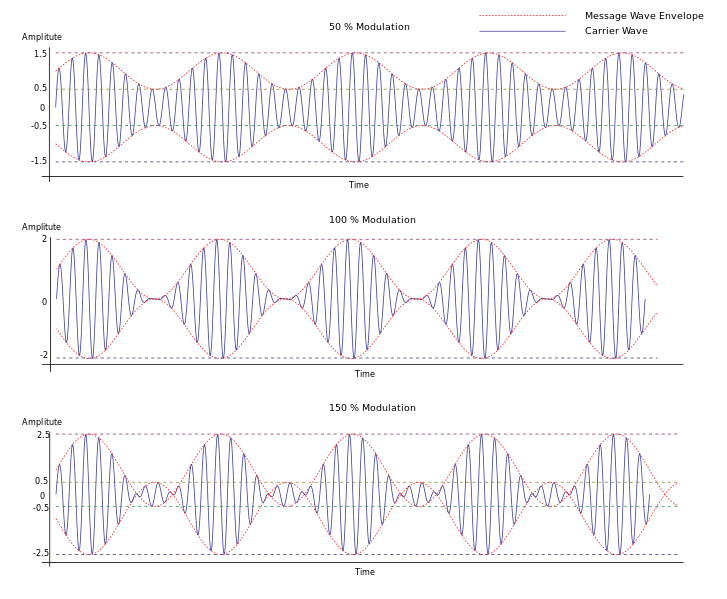
\includegraphics[width=\textwidth]{AMmodindex.png}
\caption{Effect of modulation index on AM}
\label{AMmodindex}
\end{figure}
\noindent Fig \ref{AMmodindex}  shows the effect of modulation index on the resultant AM wave\footnote{\url{https://commons.wikimedia.org:/wiki/File:Amplitude_Modulated_Wave-hm-64.svg}}
\begin{center}

\begin{tabular}{|l|l|l|}

\hline
 & &\\
 
$E_{min}$  & $E_{max}$ & $m=\frac{E_{max}-E_{min}}{E_{max}+E_{min}}$ \\
 & & \\ \hline
 & & \\ \hline
& & \\ \hline
& & \\ \hline
& & \\ \hline
& & \\ \hline

\end{tabular}
\end{center}


\section*{Result}

Implemented the AM modulation circuit using BJT.
The modulation index corresponding to $E_m=$ \textemdash \textemdash and $E_c=$ \textemdash\textemdash is : m= \textemdash\textemdash .






\chapter[Amplitude Modulation - Detection]{Amplitude Modulation - Detection}

\section*{Aim}
The experiment aims at designing an AM demodulator circuit and implementing it.

\section*{Theory}
The AM signal is a high radio frequency carrier whose amplitude envelope represents a slow varying message signal, as can be seen in Fig. \ref{AMmodindex}. The process of detecting the envelope and thus regaining the message signal from the modulated carrier wave is calledd AM demodulation.
\paragraph{}
It can be implemented by a simple diode envelope detector to eliminate the negative half of the carrier envelope followed by a simple RC filter to remove the high frequency carrier. The result will be the low frequency envelope which is the demodulated message.
\paragraph{}
A diode with low junction capacitance is used in the circuit as it is has to rectify high frequency carrier.It offers low impedence at high frequency. The \textbf{RC} circuit used at the output of the diode acts as a filter. Its time constant is chosen wisely so that it is too slow to follow the high frequency of the carrier wave at the same time its fast enough to follow the low frequency message envelope. 


\section*{Design}
Choose high frequency diode OA79.

\noindent The time period of the circuit must be much larger than the RF carrier frequency.

\begin{equation}
R_1C_1 >> T_c
\end{equation}

\begin{equation}
R_1C_1 >> \frac{1}{f_c} = \frac{1}{2\pi\omega_c}
\end{equation}

\noindent At the same time it should be smaller than the message bandwidth. ie.,

\begin{equation}
R_1C_1<< \frac{1}{f_m}
\end{equation}

\noindent Assuming $f_c=100 kHz(T_c=.01ms)$ and $f_m=1kHz(T_m=1 ms)$,
Let 
\begin{equation}
R_1C_1 = 10 X T_c =0.1 ms
\end{equation}
\noindent Let $C_1=.01\mu F$
\begin{equation}
R_1 = \frac{.1ms}{C_1} 
\end{equation}
\begin{equation}
R_1 = \frac{.1ms}{0.01\mu F}=10 k\Omega. 
\end{equation}
\section*{Circuit Diagram}

\begin{figure}[h]
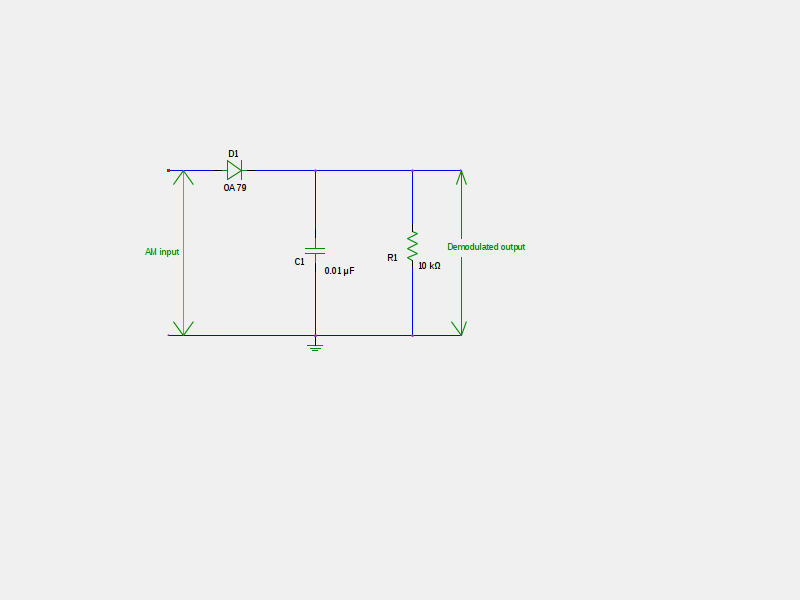
\includegraphics[width=15cm, height=10cm, trim=5cm 7.5cm 7.5cm 4cm, clip=true]{AMDemod.png}
\caption{AM Demodulation-Simple Diode Detector}
\label{AMDemod} 
\end{figure}
The circuit diagram for AM Demodulator using a simple diode detector is shown in Fig. \ref{AMDemod}.

\section*{Components and Equipments Required}
CRO, Function Generators(2), Breadboard, Probes.
\\Diodes- OA79
\\Capacitor- 0.01 $\mu$F
\\Resistor-10k$\Omega$
\section*{Procedure}

\begin{enumerate}
\item
Make connections on the breadboard as per the circuit diagram.
\item
Supply AM signal either from the signal generator or from the circuit designed in experiment Amplitude Modulation- Generation. 
\item
Connect the demodulated output to one channel of CRO along with the unmodulated signal on the other channel.
\item
Observe the Modulated and demodulated waveforms and plot it on a graph sheet.
\end{enumerate}
\section*{Observation}
A model plot showing the expected result of the experiment is shown in the Fig.\ref{AMdemod}
\begin{figure}
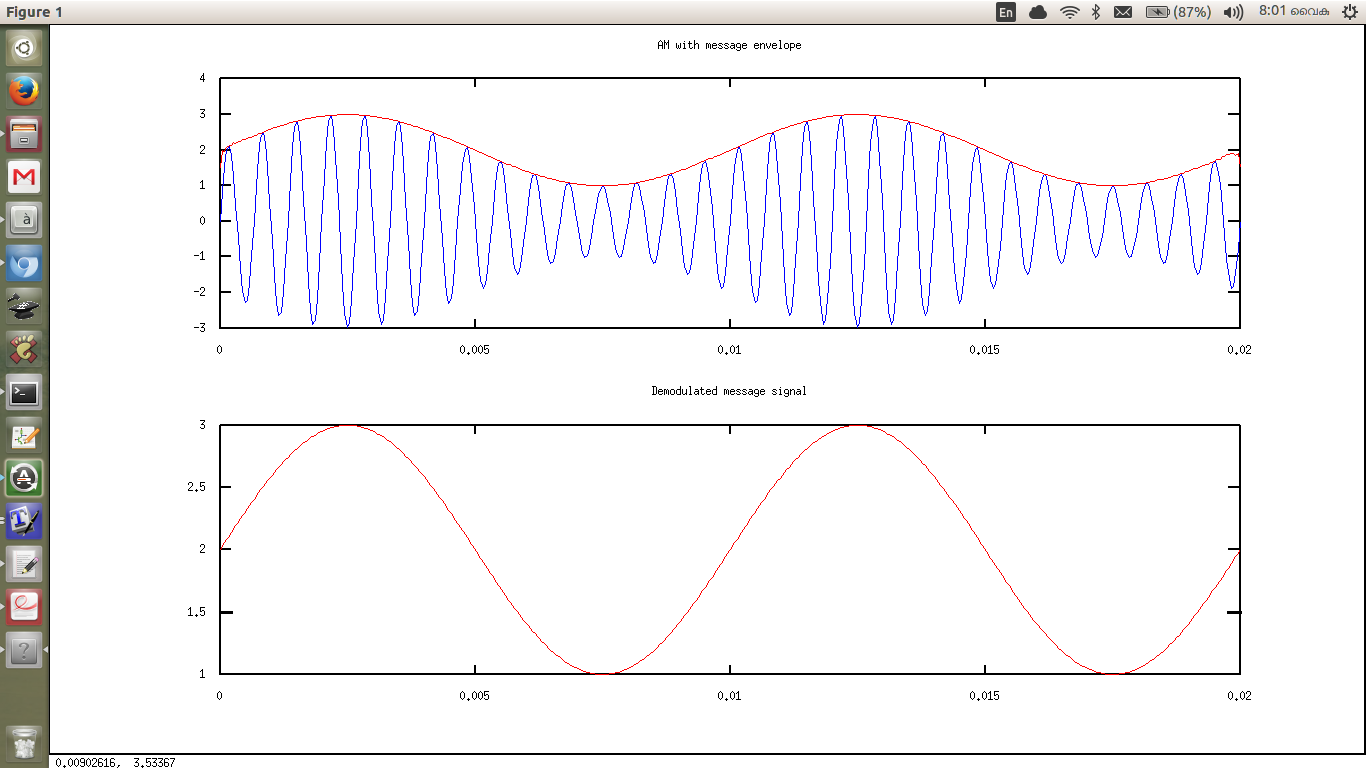
\includegraphics[width=12cm, height=10cm, trim= 2cm 1cm 1cm 1cm,clip=true]{AMdemod.png}
\caption{Modulated AM signal and Demodulated carrier}
\label{AMdemod}
\end{figure}

\section*{Result}

AM demodulation circuit was implemented on breadboard and output was observed and plotted ona graph sheet.

\chapter[Mixer Circuit using FET and BJT]{Mixer Circuit using FET and BJT}


\chapter[Balanced Modulator for DSB-SC]{Balanced Modulator for DSB-SC}
\section*{Aim}
\section*{Theory}
\section*{Design}
\section*{Circuit Diagram}
\section*{Procedure}
\section*{Observation}
\section*{Result}


\chapter[FM generation - Reactance Modulator]{FM generation - Reactance Modulator}
\section*{Aim}
\section*{Theory}
\section*{Design}
\section*{Circuit Diagram}
\section*{Procedure}
\section*{Observation}
\section*{Result}
\chapter[FM Demodulation]{FM Demodulation}
\section*{Aim}
\section*{Theory}
\section*{Design}
\section*{Circuit Diagram}
\section*{Procedure}
\section*{Observation}
\section*{Result}

\chapter[PAM Generation and Demodulation]{PAM Generation and Demodulation}
\section*{Aim}
\section*{Theory}
\section*{Design}
\section*{Circuit Diagram}
\section*{Procedure}
\section*{Observation}
\section*{Result}

\chapter[Intermediate Fequency Amplifier]{Intermediate Fequency Amplifier}
\section*{Aim}
\section*{Theory}
\section*{Design}
\section*{Circuit Diagram}
\section*{Procedure}
\section*{Observation}
\section*{Result}

\chapter[FM Demodulation using PLL]{FM Demodulation using PLL}
\section*{Aim}
\section*{Theory}
\section*{Design}
\section*{Circuit Diagram}
\section*{Procedure}
\section*{Observation}
\section*{Result}

\chapter[AM generation and Demodulation]{AM generation and Demodulation}
\section*{Aim}
\section*{Theory}
\section*{Design}
\section*{Circuit Diagram}
\section*{Procedure}
\section*{Observation}
\section*{Result}
\chapter[SSB generation and Demodulation]{SSB generation and Demodulation}
\section*{Aim}
\section*{Theory}
\section*{Design}
\section*{Circuit Diagram}
\section*{Procedure}
\section*{Observation}
\section*{Result}
\begin{appendix}
\chapter {Quick Reference-Data on Components}
\section{BJT BF194/195}
\label{BF194/195}
BF194/195 is a high frequency transistor. From its datasheet 

Type Designator: BF194/BF195

Material of transistor: Si

Polarity: NPN

Maximum collector power dissipation ($Pc$), W: 0.25

Maximum collector-base voltage |$V_{cb}$|, V: 30

Maximum collector-emitter voltage |$V_{ce}$|, V: 20

Maximum emitter-base voltage |$V_{eb}$|, V: 5

Maximum collector current |$I_{c max}$|, mA: 30

Forward current transfer ratio (hFE), min: 67

\textcolor{red}{TODO: Pinout diagram to be added}

\section{Intermediate Frequency Transformer}
\label{IFT}
IFT act as parallel resonant circuits whose resonating frequency is around 455 kHz. This frequecy is adjustable by a factor of  \textcolor{red}{FIXME} plusorminus 10\%. IFT has a tappedd primary winding and a secondary winding. Primary winding has a capacitor connected in parallel internally. Its inductor value is $L_eq=450\ mu H$ and capacitance $C=270\ pF$. 
\\Its resonant frequency is thus $f=\frac{2\pi}{\sqrt{L_{eq}C}}\approx 455 kHz$.

\textcolor{red}{TODO: add schematic diagram and photo of IFT}
\end{appendix}
\begin{thebibliography}{1}
\bibitem{ACmanual}{LABORATORY MANUAL COMMUNICATIONS LABORATORYEE 321, CALIFORNIA STATE UNIVERSITY, LOS ANGELES
Lab-Volt Systems, Inc}

\end{thebibliography}


\end{document}
